\subsection{Overview}
\label{sec:overview}
Figure \ref{fig:goat_workflow} displays the overview of \goat.
%
Given a program \textbf{P} (\ie, a set of Go source files with a \textit{main} function), \goat automatically instruments \textbf{P} and constructs static and dynamic models of execution for thorough testing and analysis.
%
Our main goal in \goat is to facilitate the investigation of \textit{non-deterministic interactions between concurrent components} (\ie, concurrent behavior) of \textbf{P} to achieve objectives acquainted in section \ref{sec:intro}.
%
\\
\noindent{\bf Static Analysis:\/} (section \ref{sec:static_analysis})---
\goat statically constructs a model \textbf{M} which is a table of source locations (files and line numbers) associated with concurrency primitive usages in \textbf{P} source files.
%
The primary use of \textbf{M} is to identify locations in \textbf{P} as potential points for manipulating the schedule to explore possible scenarios and accelerate the discovery of rare bugs.
%
Yield handlers are injected before each entry in \textbf{M} to decide if the following concurrency action (\eg, message send or mutex lock) should perform or yield to other goroutines.
%
Such yields effectively perturb the scheduler and execute feasible but unconventional interleavings of \textbf{P}.
%
\\
\noindent{\bf Coverage Requirements:\/} (section \ref{sec:covreq})---
Forcing the schedule perturbation is effective for exploring the feasible interleaving space until the bug is hit.
%
However, a metric is required to evaluate the quality of interleaving space exploration and measure the progress until reaching a threshold.
%
Following the factors of effective coverage metrics, we employ \textbf{M} to emulate the possible behavior of concurrent components of \textbf{P} and define a set of \textit{coverage requirements} as indicators for quality and progress of schedule space exploration.
%
The requirements are defined so that, during testing, a lack of requirement demands the user to fix the bug or remove the dead code.
\\
\noindent{\bf Dynamic Analysis:\/} (section \ref{sec:dynamic_tracing})---
To gain insight into the concurrent behavior of \textbf{P} and measure the covered requirements, we equipped \goat with a dynamic tracing mechanism, which is an extension to the Go standard tracer package~\cite{go-cmd-trace}.
%
When tracing is enabled, an \textit{execution concurrency trace} (ECT) file is generated once the execution of \textbf{P} terminates (\eg, successfully exits, fails, times out).
%
ECT is a totally ordered \textit{sequence} of events that contain information about the dynamic behavior concurrent components, enabling offline analysis of \textbf{P}'s execution.
\\
\noindent{\bf Offline Analysis:\/} (section \ref{sec:offline_analysis})---
In offline, \goat first, separates the application-level events of ECT from the underlying runtime system of Go.
%
Then, it constructs a goroutine tree from application-level goroutines to check if any goroutine has leaked/blocked (\ie, did not reach its final state) after the execution termination.
%
Additionally, \goat maintains a global goroutine tree for \textbf{P} and equivalences goroutines from run to run to accumulate the covered requirements from each execution of \textbf{P}.
%
As soon as a bug is detected or the coverage exceeds a threshold, \goat stops running and produces reports for manual analysis by the user.
%

\subsection{Static Analysis}
\label{sec:static_analysis}

\subsubsection{Concurrency Usage Model}
\goat statically constructs a model \textbf{M} from the usage of concurrency primitives in \textbf{P} files which enables uniform analysis during testing iterations.
%
\textbf{M} is a table of source locations (files and line numbers) associated with \textit{concurrency usages} (CU).
%
We define CU as a triple of $(f,l,k)$ where $f$ is the file name, $l$ is the line number, and $k$ is the concurrency primitive used in the code location.
$k\in$ \texttt{Channel} $\cup$ \texttt{Sync} $\cup$ \texttt{Go} where:
\begin{itemize}
  \item \texttt{Channel} = \{\texttt{send}, \texttt{receive}, \texttt{close}\}
  \item \texttt{Sync} = \{\texttt{lock}, \texttt{unlock}, \texttt{wait}, \texttt{add}, \texttt{done}, \texttt{signal}, \texttt{broadcast}\}
  \item \texttt{Go} = \{\texttt{go}, \texttt{select}, \texttt{range}\}
\end{itemize}

\goat constructs \textbf{M} by traversing the \textit{abstract syntax tree} (AST) for each file in \textbf{P} using the Go AST package~\cite{go-package-ast}.
%
The first column of table \ref{tab:moby_cov_table} shows the CU locations extracted from program in listing \ref{listing:moby28462.minipage}.

\subsubsection{Source Instrumentation}

We employ \textbf{M} entries to instrument \textbf{P} with tracing and schedule perturbation mechanisms.
%
First, we traverse the AST of \textbf{P} and inject three statements (\ie, AST nodes) to the beginning of \textbf{P}'s main function to enable end-to-end tracing:
\begin{itemize}
  \item \texttt{goat\_done := goat.Start()} initializes \goat, enables tracing, and returns a channel as a conduit between application space and \goat.
  \item \texttt{go goat.Watch(goat\_done)} spawns a new goroutine as a watchdog for the liveness of the program (in case of global deadlock or infinite loop). The watchdog goroutine either receives from \texttt{goat\_done} and sends back an ack signal or timeouts (default: 30 seconds). Then it stops tracing, flushing the trace buffer, and terminates.
  \item \texttt{defer goat.Stop(goat\_done)} sends a value to the watcher goroutine after main returns and signals that the program is finished. Then it waits to receive the signal from the watcher, then stops tracing and terminates.
\end{itemize}

Moreover, we inject calls to \texttt{goat.handler()} before each CU in \textbf{M} to manipulate the native scheduler around concurrency primitve usages. \texttt{goat.handler()} is a function invocation that randomly calls \texttt{runtime.GoSched()} within a bound $D$ to preempt the processing core from current goroutine and push the goroutine to the back of the global queue of runnable goroutines.
%
When $D=0$, \goat does not perturb the scheduler and lets \textbf{P} to execute natively. For any $D>0$, \goat manipulates application-level goroutines from their regular execution D times.
%
Our experiments (section \ref{sec:evaluation}) demonstrate that the optimum value for $D$ is not larger than 3, showing that even a small number of yields is effective in exposing the bug (as also shown in \cite{burckhardt-depthBug-asplos10}).

\subsection{Coverage Requirements}
\label{sec:covreq}
Based on our investigations from the execution of Go applications and bug kernels, we emulate the possible behavior of concurrent components by defining a set of coverage requirements (summarized in table \ref{tab:cov_req}):
%
\begin{itemize}
  \item \textbf{Req1 (Send/Recv):} \{\texttt{blocked}, \texttt{unblocking}, \texttt{NOP}\} -- Goroutine $G_1$ is either \textit{blocked} on a channel send (receive) if the receiver (sender) goroutine $G_2$ is not ready, or \textit{unblocking} the waiting receiver (sender) goroutine $G_2$. A channel send or receive might also be neither blocked nor unblocking (NOP) for buffered channels.
  \item \textbf{Req2 (Select-Case):} \{\texttt{blocked}, \texttt{unblocking}, \texttt{NOP}\} $\times$ \{\texttt{case}$_i$\} -- cases of select statements are channel sends and recives (or default case for non-blocking selects). For all select statements that has no default case, we obtain the cases of each select statement at runtime and maintain an instance of Req1 per case.
  \item \textbf{Req3 (Lock):} \{\texttt{blocked}, \texttt{blocking}\} -- Goroutine $G_i$ is either \textit{blocked} when locking a mutex because another goroutine has locked the mutex or \textit{blocking} other goroutines from acquiring the mutex lock.
  \item \textbf{Req4 (Unblocking):} \{\texttt{unblocking}, \texttt{NOP}\} -- The goroutine that is performing channel close, mutex unlock, conditional variable signal and broadcast, waitGroup done, and non-blocking select case (send or receive) either \textit{unblocks} one or more blocked goroutines or has no effect (NOP).
  \item \textbf{Req5-Go:} \{\texttt{NOP}\} -- We emit a NOP action for each goroutine creation to indicate that it is covered during testing.
\end{itemize}


\begin{table}[]
\centering
\caption{Coverge requirements defined for concurrent Go}
\scalebox{0.83}{
\begin{tabular}{|
>{\columncolor[HTML]{FFFFFF}}c |
>{\columncolor[HTML]{FFFFFF}}l |
>{\columncolor[HTML]{FFFFFF}}c |
>{\columncolor[HTML]{FFFFFF}}c |
>{\columncolor[HTML]{FFFFFF}}c |
>{\columncolor[HTML]{FFFFFF}}c |}
\hline
\cellcolor[HTML]{FFFFFF} & \multicolumn{1}{c|}{\cellcolor[HTML]{FFFFFF}} & \multicolumn{4}{c|}{\cellcolor[HTML]{FFFFFF}Coverage Requirement Types} \\ \cline{3-6}
\multirow{-2}{*}{\cellcolor[HTML]{FFFFFF}\begin{tabular}[c]{@{}c@{}}Coverage\\ Requirements\end{tabular}} & \multicolumn{1}{c|}{\multirow{-2}{*}{\cellcolor[HTML]{FFFFFF}\begin{tabular}[c]{@{}c@{}}Concurrent\\ Action\end{tabular}}} & Blocked & Unblocking & Blocking & NOP \\ \hline \hline
\cellcolor[HTML]{FFFFFF} & SEND & * & * &  & * \\ \cline{2-6}
\multirow{-2}{*}{\cellcolor[HTML]{FFFFFF}Req1: Send/Recv} & RECV & * & * &  & * \\ \hline
\cellcolor[HTML]{FFFFFF} & C$_i$ (SEND) & * & * &  & * \\ \cline{2-6}
\multirow{-2}{*}{\cellcolor[HTML]{FFFFFF}Req 2: Select-Case} & C$_i$ (RECV) & * & * &  & * \\ \hline
Req 3: Lock & LOCK & * &  & * &  \\ \hline
\cellcolor[HTML]{FFFFFF} & CLOSE &  & * &  & * \\ \cline{2-6}
\cellcolor[HTML]{FFFFFF} & UNLOCK &  & * &  & * \\ \cline{2-6}
\cellcolor[HTML]{FFFFFF} & SIGNAL &  & * &  & * \\ \cline{2-6}
\cellcolor[HTML]{FFFFFF} & BRDCST &  & * &  & * \\ \cline{2-6}
\multirow{-5}{*}{\cellcolor[HTML]{FFFFFF}Req 4: Unblocking} & SELECT-DEF &  & * &  & * \\ \hline
Go & GO &  &  &  & * \\ \hline
\end{tabular}

}
\label{tab:cov_req}
\end{table}

%
With the help of \goat's infrastructure, the proposed requirements satisfy the characteristics of an ``acceptable'' coverage metric because:
\begin{enumerate}
  \item A \textit{static model} \textbf{M} from program \textbf{P} is obtained by identifying its CU points. \textbf{M} is easy to understand by developers and reflects the concurrent behavior of \textbf{P}.
  \item The defined requirements are \textit{measurable} by analyzing the test's ECT. A global data structure maintains the covered requirements by each $t \in \mathcal{T}$.
  \item Upon completion of $\mathcal{T}$ iterations, the \textit{uncovered} requirements imply some \textit{meaningful} information about the behavior of \textbf{P}. For example, if a send is always performing as \textit{unblocking} and never as \textit{blocked}, it means that the receiver always performs receive before the sender reaches its send instruction. In other words, the receive action \textit{always happen-before} send action. This communication pattern might be part of \textbf{P}'s semantics and matches the developer's expectations (e.g., a set of goroutines are listening on a channel to perform non-frequent requests). Otherwise, the uncovered requirement  ``send-\texttt{blocked}'' reflects a bug or flaw in the program design.
  \item Since \goat can detect occurred blocking bugs and maintain a global coverage model, $\mathcal{T}$ iterations terminate either by detecting a bug or reaching a coverage percentage threshold.
\end{enumerate}

\subsection{Dynamic Concurrency Tracing}
\label{sec:dynamic_tracing}
The standard execution tracer package \cite{go-package-trace,go-cmd-trace} provides dynamic tracing for the construction of execution models from the interactions of processors, OS threads, goroutines, the scheduler, and the garbage collection mechanism.
%
The tracing mechanism is compiled into all programs always through the runtime and is enabled on demand to study \textit{perfromance bottlenecks} through visualizers like \textit{pprof} \cite{go-profile-blog}.
%
The alphabet of trace events is total of 49 events \cite{goParserSource}, categorized and summarized in table \ref{tab:events}.
%
Although the event vocabulary is rich enough to model comprehensive goroutine latency and blocking behavior accurately,
the vocabulary lacks concurrency primitive usage events for the construction of concurrency models.
%
We enrich the standard tracing mechanism with 14 additional events to enable the production of dynamic models from the program's concurrency behavior:
\begin{itemize}
    \item \textbf{Channel:} For each channel operation (make, send, receive, close), ECT includes an event with a unique id assigned to each channel.
    \item \textbf{(RW)Mutex, WaitGroup \& Conditional Variables:} Similar to channels, we assign a unique id to each concurrency object and emit an event for each of their operations (lock, unlock, rlock, runlock, add, wait, signal, broadcast).
    \item \textbf{Select \& Schedule:} The scheduler and the \textit{select} structure introduce non-determinism to the execution. We keep track of the decisions made by the scheduler and select statements to obtain an accurate decision path during execution.
\end{itemize}

We call the output of enhanced tracer \textit{execution concurrency trace} (ECT).
%
ECT is a totally ordered \textit{sequence} of events in which the order is approximated through a central clock with nanosecond precision.
%
ECT also contains the call-stack for each event, enabling a direct mapping of events to source-line numbers.
%
For each blocking operation (channels \textit{sends}/\textit{recvs}, mutex \textit{locks}, waitGroup/conditional variable \textit{wait} and \textit{select} (when none of the cases are available)), ECT captures a pair of pre-operation and post-operation events to distinguish between the \textit{request for action} and \textit{completion of action}.
%
Hence, ECT is especially effective for debugging because it enables modeling the blocking state of concurrent components at any given step of program execution.
%
The enhanced dynamic tracing also enables the measurement of coverage requirements in offline (section \ref{sec:offline_analysis}).

\begin{table}[]
    \centering
        \caption{Event categories by the Go execution tracer}
        \begin{tabular}{|l|l|}
        \hline
        \rowcolor[HTML]{C0C0C0}
        \multicolumn{1}{|c|}{\cellcolor[HTML]{C0C0C0}\textbf{Category}} & \multicolumn{1}{c|}{\cellcolor[HTML]{C0C0C0}\textbf{Description}} \\ \hline
        Process & Indication of process/thread start and stop \\ \hline
        GC/Mem & Garbage collection and memory operation events\\ \hline
        Goroutine & Goroutines events: create, block, start, stop, end, etc. \\ \hline
        Syscall & Interactions with system calls \\ \hline
        Users & User annotated regions and tasks (for bounded tracing) \\ \hline
        Misc & System related events like futile wakeup or timers \\ \hline
        \end{tabular}
    \label{tab:events}
\end{table}



\subsection{Offline Analysis}
\label{sec:offline_analysis}
In the lifetime of Go programs' executions, the runtime system creates new goroutines or pick from the pool of dead goroutines to perform various tasks such as bootstrapping the program, garbage marking and sweeping, and tracing.
%
\goat also adds an extra goroutine to \textit{watch} the program execution in case of the main goroutine blockage.
%
These goroutines are captured during tracing, but our focus is on the goroutines created from within the application.
%
The distinguishment between runtime goroutines and application goroutines is essential to define the boundaries of the application and separate them from the underlying system.
%
We say a goroutine is an \textit{application-level} goroutine if it is the main goroutine (that executes the main function) or it has all of the following conditions:
1) its ancestor is the main goroutine,
2) it is not a Go runtime system goroutine, and
3) it is not a tracer goroutine.
These conditions are assessed for every captured goroutine in ECT by checking the call stack of their corresponding $GoCreate$ event.

\goat constructs a \textit{goroutine tree} (figure \ref{fig:gtree}) of application-level goroutines from the generated ECT.
%
Nodes in the goroutine tree represent a goroutine, and directed edges denote parent-child relationships in which the child is created from a \texttt{go} statement that the parent executes.
%
Each node of the tree contains the entire sequence of events that the goroutine executed (not shown in the figure for simplicity), information about the goroutine's creation site, the resources it holds at each execution point, and the final executed event right before the program termination.
%
\goat analyzes this collection of information to check whether any goroutine leaked after termination and whether the coverage requirements are covered.

\subsubsection{Leak Detection}
When tracing is enabled, every application goroutine invokes the tracer to capture $GoEnd$ before finishing its execution.
%
Before the main function returns, the main goroutine hands over the control to the root goroutine to finalize the program termination.
%
This context-switch is done through invocation of \texttt{runtime.Gosched()} which emits the $GoSched$ event.
%
In \goat, the main goroutine's final event in a successful execution is $GoSched$ with \texttt{runtime.traceStop} on top of its stack.

\begin{figure}[]
\centering
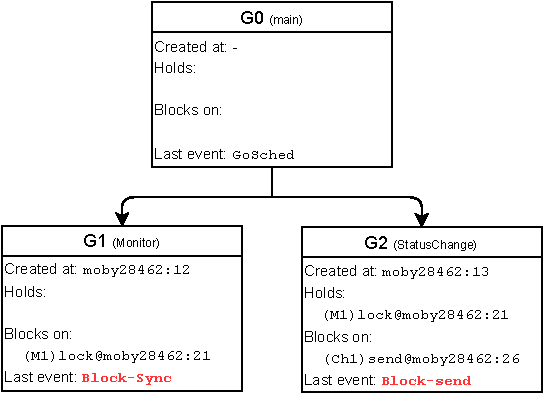
\includegraphics[width=0.75\linewidth]{figs/gtree.pdf}
%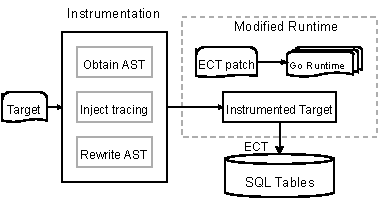
\includegraphics[]{figs/overview.png}
%\includegraphics[]{figs/overv}
\caption{Goroutine tree of the leak situation in listing \ref{listing:moby28462.minipage}}
\label{fig:gtree}
\end{figure}

We call an execution \textbf{successful}, if below conditions hold:
\begin{enumerate}
  \item (1) all goroutines spawned in the main goroutine has $GoEnd$ as their final event
  \item (2) the final event of the main goroutine is $GoSched$ with \texttt{runtime.traceStop} on top of its stack.
\end{enumerate}

In the absence of any of these conditions, we conclude that the program suffers from a ``deadlock'' bug, because at least one goroutine did not reach its final state.
%
Therefore, \goat executes procedure \ref{proc:deadlockCheck} which is a BFS traversal on the goroutine tree to check if the program suffers from partial or global deadlocks.


\begin{small}
\begin{algorithm}[]
 \DontPrintSemicolon
 \SetKwFunction{KwDeadlockCheck}{DeadlockCheck}
% \SetKwInOut{Input}{Input} \SetKwInOut{Output}{Output}\SetKwInOut{Local}{Local}
  %\SetKw{KwEach}{each}
 %\Input{Stack of elements $S$, $S[1]$ is top}
 %\Output{$NLR(T)$}
 \KwDeadlockCheck{$G$}:{\\
 \Indp
    \If{$cur$.lastEvent$ \neq$ \texttt{GoSched}}{
      return \textbf{Global Deadlock}\;
    }
    $toVisit$ = $[G.children]$\;
    \For{ $|toVisit| \neq 0$}{
         $cur$ = $toVisit$[0]\;
         \If{$cur$.lastEvent $\neq$ \texttt{GoEnd}}{
            return \textbf{Partial Deadlock (leak)}\;
          }
         \For {$n$ in $cur.Children$}{
            append $n$ to $toVisit$\;
          }
          $toVisit = toVisit[1:]$\;
      }
      return \textbf{Pass}\;
  }
 \caption{\texttt{DeadlockCheck} procedure with root node of goroutine tree (main goroutine) as input}
 \label{proc:deadlockCheck}
\end{algorithm}
\end{small}


\begin{table}[]
\centering
\caption{Concurrency Usages and coverage requirements of program in listing\ref{listing:moby28462.minipage}}
\scalebox{0.9}{

\begin{tabular}{
>{\columncolor[HTML]{FFFFFF}}c
>{\columncolor[HTML]{FFFFFF}}l |
>{\columncolor[HTML]{FFFFFF}}l |
>{\columncolor[HTML]{FFFFFF}}c |
>{\columncolor[HTML]{FFFFFF}}c |
>{\columncolor[HTML]{FFFFFF}}c |}
\hline
\multicolumn{2}{|c|}{\cellcolor[HTML]{FFFFFF}CU of list. \ref{listing:moby28462.minipage}} & \multicolumn{1}{c|}{\cellcolor[HTML]{FFFFFF}} & \multicolumn{2}{c|}{\cellcolor[HTML]{FFFFFF}Covered by} & \cellcolor[HTML]{FFFFFF} \\ \cline{1-2} \cline{4-5}
\multicolumn{1}{|c|}{\cellcolor[HTML]{FFFFFF}Line} & \multicolumn{1}{c|}{\cellcolor[HTML]{FFFFFF}Kind} & \multicolumn{1}{c|}{\multirow{-2}{*}{\cellcolor[HTML]{FFFFFF}Coverage Requirements}} & run \#1 & run \#2 & \multirow{-2}{*}{\cellcolor[HTML]{FFFFFF}\begin{tabular}[c]{@{}c@{}}Overall\\      Covered\end{tabular}} \\ \hline
\multicolumn{1}{|c|}{\cellcolor[HTML]{FFFFFF}12} & go & covered & $\checkmark_{G0}$ & $\checkmark_{G0}$ & $\checkmark$ \\ \hline
\multicolumn{1}{|c|}{\cellcolor[HTML]{FFFFFF}13} & go & covered & $\checkmark_{G0}$ & $\checkmark_{G0}$ & $\checkmark$ \\ \hline
\multicolumn{1}{|c|}{\cellcolor[HTML]{FFFFFF}} & \cellcolor[HTML]{FFFFFF} & c-recv-blocked & $\checkmark_{G1}$ &  & $\checkmark$ \\ \cline{3-6}
\multicolumn{1}{|c|}{\multirow{-2}{*}{\cellcolor[HTML]{FFFFFF}17}} & \multirow{-2}{*}{\cellcolor[HTML]{FFFFFF}select} & c-recv-unblocking & $\checkmark_{G1}$ &  & $\checkmark$ \\ \hline
\multicolumn{1}{|c|}{\cellcolor[HTML]{FFFFFF}} & \cellcolor[HTML]{FFFFFF} & blocked &  & \cellcolor[HTML]{C0C0C0}$\checkmark_{G1}$ & $\checkmark$ \\ \cline{3-6}
\multicolumn{1}{|c|}{\multirow{-2}{*}{\cellcolor[HTML]{FFFFFF}21}} & \multirow{-2}{*}{\cellcolor[HTML]{FFFFFF}lock} & blocking & $\checkmark_{G1}$ &  & $\checkmark$ \\ \hline
\multicolumn{1}{|c|}{\cellcolor[HTML]{FFFFFF}} & \cellcolor[HTML]{FFFFFF} & unblocking & $\checkmark_{G1}$ &  & $\checkmark$ \\ \cline{3-6}
\multicolumn{1}{|c|}{\multirow{-2}{*}{\cellcolor[HTML]{FFFFFF}22}} & \multirow{-2}{*}{\cellcolor[HTML]{FFFFFF}unlock} & no\_op &  &  &  \\ \hline
\multicolumn{1}{|c|}{\cellcolor[HTML]{FFFFFF}} & \cellcolor[HTML]{FFFFFF} & blocked & $\checkmark_{G2}$ &  & $\checkmark$ \\ \cline{3-6}
\multicolumn{1}{|c|}{\multirow{-2}{*}{\cellcolor[HTML]{FFFFFF}25}} & \multirow{-2}{*}{\cellcolor[HTML]{FFFFFF}lock} & blocking &  & \cellcolor[HTML]{C0C0C0} \textbf{$\checkmark_{G2}$} & $\checkmark$ \\ \hline
\multicolumn{1}{|c|}{\cellcolor[HTML]{FFFFFF}} & \cellcolor[HTML]{FFFFFF} & blocked & $\checkmark_{G2}$ & $\checkmark_{G2}$ & $\checkmark$ \\ \cline{3-6}
\multicolumn{1}{|c|}{\cellcolor[HTML]{FFFFFF}} & \cellcolor[HTML]{FFFFFF} & unblocking &  &  &  \\ \cline{3-6}
\multicolumn{1}{|c|}{\multirow{-3}{*}{\cellcolor[HTML]{FFFFFF}26}} & \multirow{-3}{*}{\cellcolor[HTML]{FFFFFF}send} & no\_op &  &  &  \\ \hline
\multicolumn{1}{|c|}{\cellcolor[HTML]{FFFFFF}} & \cellcolor[HTML]{FFFFFF} & unblocking &  &  &  \\ \cline{3-6}
\multicolumn{1}{|c|}{\multirow{-2}{*}{\cellcolor[HTML]{FFFFFF}27}} & \multirow{-2}{*}{\cellcolor[HTML]{FFFFFF}unlock} & no\_op & $\checkmark_{G2}$ &  & $\checkmark$ \\ \hline
\multicolumn{1}{l}{\cellcolor[HTML]{FFFFFF}} &  & Coverage \% & 60\% & 33\% & 73\% \\ \cline{3-6}
\end{tabular}

}
\label{tab:moby_cov_table}
\end{table}


%\stcmt{reports and visualizations}
When a deadlock is detected, \goat generates visualizations such as executed interleaving (listing \ref{listing:moby28462.minipage}) and goroutine tree (figure \ref{fig:gtree}).
%
The detailed report magnifies the scenario under which the bug has occurred and displays the final concurrent state of the program right before the failure.
%
In addition, custom logs and reports such as the ``happens-before'' log of a set of goroutines and their associated resources are easily generated through a replay of ECT.
%
Samples of such reports and visualizations are available in [appendix or online link]

\subsubsection{Coverage Measurement}
Once the program execution terminates, \goat checks whether the extracted coverage requirements are covered during execution.
%
A mapping between ECT dynamic concurrent events and statically obtained CU points is emitted by matching their respective call-stack and CU source location.
%
Through a BFS traversal of the goroutine tree, we add a \textit{coverage vector} to each goroutine node from the emitted mapping.
%
Each element of the coverage vector is the respective covered value of the coverage requirement for the current goroutine node.
%
During executions of tests $t \in \mathcal{T}$, we maintain and update a global goroutine tree after each $t$.
%
It is crucial to maintain a global goroutine tree to measure the progress of coverage percentage over tests in $\mathcal{T}$.
%
However, equivalencing between two goroutines and their respective coverage vectors from different executions is non-trivial.
%
We say two goroutines $G_m$ and $G_n$ in the tests $t_i$ and $t_j$ are \textit{equivalent} (\ie falls into a identical node in the global goroutine tree) if their parents are equivalent and their creation source location (CU of kind \texttt{go}) are identical.
%
\begin{equation}
  G_m \equiv G_n   \text{if}
  \begin{cases}
    \text{parent}(G_m) \equiv \text{parent}(G_n)  \wedge \\
    \text{CU(}G_m\text{).file} = \text{CU(}G_n\text{).file}  \wedge\\
    \text{CU(}G_m\text{).line} = \text{CU(}G_n\text{).line} \\
  \end{cases}
\end{equation}


\begin{table*}[]
\caption{Output of each tool on GoKer \cite{yuan-gobench-cgo21} blocking bugs. Detected bug (minimum \# of executions required) -- \textbf{X (1000)}: the tool is not able to detect any bug after 1000 executions. \textbf{PDL}: Partial Deadlock, \textbf{GDL}: Global Deadlock, \textbf{PDL-k}: Partial Deadlock with \textit{k} number of goroutines leaked. \textbf{DL}: A warning for potential deadlock is issued. \textbf{TO/GDL}: The global deadlock is detected because none of goroutines made any progress after 20 seconds, \textbf{CRASH}: The execution paniced because of a flaw in the execution (e.g., send on closed channel panic), \textbf{HANG}: The tool halt for more than 10 minutes.}
\centering
\scalebox{0.72}{
    % Please add the following required packages to your document preamble:
% \usepackage{multirow}
% \usepackage[table,xcdraw]{xcolor}
% If you use beamer only pass "xcolor=table" option, i.e. \documentclass[xcolor=table]{beamer}
\begin{tabular}{|c|c|c|ccc|ccccc|}
\hline
\multicolumn{3}{|c|}{Bug Description} & \multicolumn{8}{c|}{Debugging Tools} \\ \hline
 &  &  & \multicolumn{1}{c|}{} & \multicolumn{1}{c|}{} &  & \multicolumn{5}{c|}{GOAT} \\ \cline{7-11}
\multirow{-2}{*}{Cause} & \multirow{-2}{*}{SubCause} & \multirow{-2}{*}{Bug ID} & \multicolumn{1}{c|}{\multirow{-2}{*}{BUILTINDL}} & \multicolumn{1}{c|}{\multirow{-2}{*}{GOLEAK}} & \multirow{-2}{*}{LOCKDL} & \multicolumn{1}{c|}{D0} & \multicolumn{1}{c|}{D1} & \multicolumn{1}{c|}{D2} & \multicolumn{1}{c|}{D3} & D4 \\ \hline
 &  & cockroach\_2448 & X (1000) & X (1000) & X (1000) & CRASH (1) & CRASH (1) & CRASH (1) & CRASH (1) & CRASH (1) \\ \cline{3-3}
 &  & cockroach\_24808 & GDL (1) & GDL (1) & TO/GDL (1) & TO/GDL (1) & TO/GDL (1) & TO/GDL (1) & TO/GDL (1) & TO/GDL (1) \\ \cline{3-3}
 &  & cockroach\_25456 & GDL (1) & GDL(1) & TO/GDL (1) & TO/GDL (1) & TO/GDL (1) & TO/GDL (1) & TO/GDL (1) & TO/GDL (1) \\ \cline{3-3}
 &  & cockroach\_35073 & GDL (1) & GDL (1) & TO/GDL (1) & TO/GDL (1) & TO/GDL (1) & TO/GDL (1) & TO/GDL (1) & TO/GDL (1) \\ \cline{3-3}
 &  & cockroach\_35931 & GDL (1) & GDL (1) & TO/GDL (1) & TO/GDL (1) & TO/GDL (1) & TO/GDL (1) & TO/GDL (1) & TO/GDL (1) \\ \cline{3-3}
 &  & etcd\_6857 & X (1000) & PDL (325) & X (1000) & \cellcolor[HTML]{EFEFEF}PDL-1 (1) & \cellcolor[HTML]{EFEFEF}PDL-1 (1) & \cellcolor[HTML]{EFEFEF}PDL-1 (11) & \cellcolor[HTML]{EFEFEF}PDL-1 (3) & \cellcolor[HTML]{EFEFEF}PDL-1 (3) \\ \cline{3-3}
 &  & grpc\_1275 & X (1000) & PDL (1) & X (1000) & PDL-1 (1) & PDL-1 (1) & PDL-1 (1) & PDL-1 (1) & PDL-1 (1) \\ \cline{3-3}
 &  & grpc\_1424 & X (1000) & PDL (1) & X (1000) & PDL-1 (1) & PDL-1 (1) & PDL-1 (1) & PDL-1 (1) & PDL-1 (1) \\ \cline{3-3}
 &  & grpc\_660 & X (1000) & PDL (1) & X (1000) & PDL-1 (1) & PDL-1 (1) & PDL-1 (1) & PDL-1 (1) & PDL-1 (1) \\ \cline{3-3}
 &  & istio\_17860 & X (1000) & PDL (1) & X (1000) & PDL-1 (2) & PDL-1 (1) & PDL-1 (1) & PDL-1 (1) & PDL-1 (1) \\ \cline{3-3}
 &  & kubernetes\_38669 & X (1000) & PDL (1) & X (1000) & PDL-1 (1) & PDL-1 (1) & PDL-1 (1) & PDL-1 (1) & PDL-1 (1) \\ \cline{3-3}
 &  & kubernetes\_5316 & X (1000) & PDL (1) & X (1000) & PDL-1 (1) & PDL-2 (1) & PDL-1 (1) & PDL-2 (1) & PDL-2 (1) \\ \cline{3-3}
 &  & kubernetes\_70277 & GDL (1) & GDL (1) & TO/GDL (1) & TO/GDL (1) & TO/GDL (1) & TO/GDL (1) & TO/GDL (1) & TO/GDL (1) \\ \cline{3-3}
 &  & moby\_21233 & X (1000) & PDL (1) & X (1000) & PDL-2 (1) & PDL-2 (1) & PDL-2 (1) & PDL-2 (1) & PDL-2 (1) \\ \cline{3-3}
 &  & moby\_33293 & X (1000) & PDL (1) & X (1000) & PDL-1 (1) & PDL-1 (3) & PDL-1 (1) & PDL-1 (1) & PDL-1 (1) \\ \cline{3-3}
 &  & moby\_4395 & X (1000) & PDL (1) & X (1000) & PDL-1 (1) & PDL-1 (1) & PDL-1 (1) & PDL-1 (1) & PDL-1 (1) \\ \cline{3-3}
 & \multirow{-17}{*}{Channel} & syncthing\_5795 & GDL (1) & GDL (1) & TO/GDL (1) & TO/GDL (1) & TO/GDL (1) & TO/GDL (1) & TO/GDL (1) & TO/GDL (1) \\ \cline{2-11}
 &  & kubernetes\_11298 & X (1000) & X (1000) & TO/GDL (179) & X (1000) & TO/GDL (352) & TO/GDL (158) & TO/GDL (179) & TO/GDL (179) \\ \cline{3-3}
 & \multirow{-2}{*}{\begin{tabular}[c]{@{}c@{}}Channel   \&\\      Conditional Variable\end{tabular}} & moby\_27782 & X (1000) & PDL (741) & X (1000) & X (1000) & \cellcolor[HTML]{EFEFEF}PDL-2 (1) & \cellcolor[HTML]{EFEFEF}PDL-2 (1) & \cellcolor[HTML]{EFEFEF}PDL-2 (4) & \cellcolor[HTML]{EFEFEF}PDL-2 (4) \\ \cline{2-11}
 &  & cockroach\_10790 & X (1000) & PDL (3) & X (1000) & PDL-2 (1) & PDL-2 (1) & PDL-2 (1) & PDL-2 (1) & PDL-2 (1) \\ \cline{3-3}
 &  & cockroach\_13197 & X (1000) & PDL (1) & X (1000) & PDL-1 (1) & PDL-1 (1) & PDL-1 (1) & PDL-1 (1) & PDL-1 (1) \\ \cline{3-3}
 &  & cockroach\_13755 & X (1000) & PDL (1) & X (1000) & PDL-1 (1) & PDL-1 (1) & PDL-1 (1) & PDL-1 (1) & PDL-1 (1) \\ \cline{3-3}
 &  & cockroach\_18101 & X (1000) & PDL (1) & X (1000) & PDL-1 (1) & PDL-1 (1) & PDL-1 (1) & PDL-1 (1) & PDL-1 (1) \\ \cline{3-3}
 &  & grpc\_862 & X (1000) & PDL (1) & X (1000) & PDL-1 (1) & PDL-1 (1) & PDL-1 (1) & PDL-1 (1) & PDL-1 (1) \\ \cline{3-3}
 &  & istio\_18454 & X (1000) & PDL (13) & X (1000) & PDL-2 (5) & PDL-1 (14) & PDL-1 (4) & PDL-1 (6) & PDL-1 (6) \\ \cline{3-3}
 &  & kubernetes\_25331 & X (1000) & PDL (1) & X (1000) & PDL-1 (1) & PDL-1 (1) & PDL-1 (1) & PDL-1 (1) & PDL-1 (1) \\ \cline{3-3}
 & \multirow{-8}{*}{\begin{tabular}[c]{@{}c@{}}Channel \& \\      Context\end{tabular}} & moby\_33781 & X (1000) & PDL (1) & X (1000) & PDL-1 (221) & PDL-1 (10) & PDL-1 (8) & PDL-1 (10) & PDL-1 (10) \\ \cline{2-11}
 &  & moby\_29733 & GDL (1) & GDL (1) & TO/GDL (1) & TO/GDL (1) & TO/GDL (1) & TO/GDL (1) & TO/GDL (1) & TO/GDL (1) \\ \cline{3-3}
\multirow{-29}{*}{\begin{tabular}[c]{@{}c@{}}Communication\\       Deadlock\end{tabular}} & \multirow{-2}{*}{Condition Variable} & moby\_30408 & GDL (1) & GDL (1) & TO/GDL (1) & TO/GDL (1) & TO/GDL (1) & TO/GDL (1) & TO/GDL (1) & TO/GDL (1) \\ \hline
 &  & etcd\_6873 & X (1000) & PDL (371) & X (1000) & PDL-2 (1) & PDL-2 (2) & PDL-2 (7) & PDL-2 (6) & PDL-2 (6) \\ \cline{3-3}
 &  & etcd\_7443 & X (1000) & X (1000) & X (1000) & X (1000) & \cellcolor[HTML]{EFEFEF}PDL-1 (9) & \cellcolor[HTML]{EFEFEF}PDL-1 (15) & \cellcolor[HTML]{EFEFEF}PDL-1 (14) & \cellcolor[HTML]{EFEFEF}PDL-1 (14) \\ \cline{3-3}
 &  & etcd\_7492 & HANG (1) & HANG (1) & TO/GDL (4) & TO/GDL (1) & TO/GDL (1) & TO/GDL (1) & TO/GDL (1) & TO/GDL (1) \\ \cline{3-3}
 &  & etcd\_7902 & X (1000) & PDL (1) & X (1000) & PDL-4 (1) & PDL-4 (1) & PDL-4 (1) & PDL-4 (1) & PDL-4 (1) \\ \cline{3-3}
 &  & grpc\_1353 & X (1000) & PDL (1) & X (1000) & CRASH (1) & CRASH (1) & PDL-3 (1) & PDL-3 (1) & PDL-3 (1) \\ \cline{3-3}
 &  & grpc\_1460 & X (1000) & PDL (1) & X (1000) & PDL-2 (135) & PDL-2 (1) & PDL-2 (2) & PDL-2 (1) & PDL-2 (1) \\ \cline{3-3}
 &  & istio\_16224 & GDL (1) & GDL (1) & TO/GDL (1) & TO/GDL (1) & TO/GDL (1) & TO/GDL (1) & TO/GDL (1) & TO/GDL (1) \\ \cline{3-3}
 &  & kubernetes\_10182 & X (1000) & PDL (44) & X (1000) & \cellcolor[HTML]{EFEFEF}PDL-2 (1) & \cellcolor[HTML]{EFEFEF}PDL-2 (1) & \cellcolor[HTML]{EFEFEF}PDL-2 (1) & \cellcolor[HTML]{EFEFEF}PDL-2 (1) & \cellcolor[HTML]{EFEFEF}PDL-2 (1) \\ \cline{3-3}
 &  & kubernetes\_1321 & X (1000) & PDL (307) & X (1000) & X (1000) & \cellcolor[HTML]{EFEFEF}PDL-1 (1) & \cellcolor[HTML]{EFEFEF}PDL-1 (1) & \cellcolor[HTML]{EFEFEF}PDL-1 (1) & \cellcolor[HTML]{EFEFEF}PDL-1 (1) \\ \cline{3-3}
 &  & kubernetes\_26980 & GDL (375) & GDL (131) & X (1000) & TO/GDL (191) & TO/GDL (1) & TO/GDL (1) & TO/GDL (1) & TO/GDL (1) \\ \cline{3-3}
 &  & kubernetes\_6632 & X (1000) & X (1000) & X (1000) & \cellcolor[HTML]{EFEFEF}PDL-2 (1) & \cellcolor[HTML]{EFEFEF}PDL-2 (1) & \cellcolor[HTML]{EFEFEF}PDL-2 (2) & \cellcolor[HTML]{EFEFEF}PDL-2 (1) & \cellcolor[HTML]{EFEFEF}PDL-2 (1) \\ \cline{3-3}
 &  & moby\_28462 & X (1000) & PDL (5) & X (1000) & PDL-2 (39) & PDL-2 (1) & PDL-2 (1) & PDL-2 (1) & PDL-2 (1) \\ \cline{3-3}
 & \multirow{-13}{*}{Channel \& Lock} & serving\_2137 & X (1000) & X (1000) & X (1000) & X (1000) & X (1000) & TO/GDL (88) & X (1000) & X (1000) \\ \cline{2-11}
 &  & cockroach\_1055 & GDL (1) & GDL (1) & TO/GDL (1) & TO/GDL (1) & TO/GDL (1) & TO/GDL (1) & TO/GDL (1) & TO/GDL (1) \\ \cline{3-3}
 & \multirow{-2}{*}{\begin{tabular}[c]{@{}c@{}}Channel   \& \\      WaitGroup\end{tabular}} & cockroach\_1462 & X (1000) & X (1000) & TO/GDL (1) & X (1000) & TO/GDL (1) & TO/GDL (1) & TO/GDL (1) & TO/GDL (1) \\ \cline{2-11}
\multirow{-16}{*}{\begin{tabular}[c]{@{}c@{}}Mixed \\      Deadlock\end{tabular}} & Misuse WaitGroup & moby\_25384 & X (1000) & PDL (1) & X (1000) & PDL-1 (1) & PDL-1 (1) & PDL-1 (1) & PDL-1 (1) & PDL-1 (1) \\ \hline
 &  & cockroach\_584 & X (1000) & PDL (1) & X (1000) & PDL-1 (1) & PDL-1 (1) & PDL-1 (1) & PDL-1 (1) & PDL-1 (1) \\ \cline{3-3}
 &  & cockroach\_9935 & X (1000) & PDL (1) & DL (721) & PDL-1 (1) & PDL-1 (2) & PDL-1 (1) & PDL-1 (1) & PDL-1 (1) \\ \cline{3-3}
 &  & etcd\_10492 & GDL (1) & GDL (1) & DL (1) & TO/GDL (1) & TO/GDL (1) & TO/GDL (1) & TO/GDL (1) & TO/GDL (1) \\ \cline{3-3}
 &  & etcd\_5509 & X (1000) & GDL (766) & TO/GDL (426) & X (1000) & TO/GDL (1) & TO/GDL (1) & TO/GDL (1) & TO/GDL (1) \\ \cline{3-3}
 &  & etcd\_6708 & GDL (1) & GDL (1) & DL (1) & TO/GDL (1) & TO/GDL (1) & TO/GDL (1) & TO/GDL (1) & TO/GDL (1) \\ \cline{3-3}
 &  & grpc\_3017 & GDL (4) & GDL (4) & TO/GDL (3) & TO/GDL (1) & TO/GDL (1) & TO/GDL (1) & TO/GDL (1) & TO/GDL (1) \\ \cline{3-3}
 &  & grpc\_795 & GDL (1) & GDL (1) & DL (1) & TO/GDL (1) & TO/GDL (1) & TO/GDL (1) & TO/GDL (1) & TO/GDL (1) \\ \cline{3-3}
 &  & hugo\_5379 & GDL (1) & GDL (1) & TO/GDL (1) & TO/GDL (1) & TO/GDL (1) & TO/GDL (1) & TO/GDL (1) & TO/GDL (1) \\ \cline{3-3}
 &  & moby\_17176 & X (1000) & PDL (1) & X (1000) & PDL-1 (1) & PDL-1 (1) & PDL-1 (1) & PDL-1 (1) & PDL-1 (1) \\ \cline{3-3}
 &  & moby\_36114 & X (1000) & PDL (1) & X (1000) & PDL-1 (1) & PDL-1 (1) & PDL-1 (1) & PDL-1 (1) & PDL-1 (1) \\ \cline{3-3}
 &  & moby\_7559 & X (1000) & PDL (1) & X (1000) & PDL-1 (1) & PDL-1 (1) & PDL-1 (1) & PDL-1 (1) & PDL-1 (1) \\ \cline{3-3}
 & \multirow{-12}{*}{Double locking} & syncthing\_4829 & GDL (1) & GDL (1) & DL (1) & TO/GDL (1) & TO/GDL (1) & TO/GDL (1) & TO/GDL (1) & TO/GDL (1) \\ \cline{2-11}
 &  & cockroach\_16167 & X (1000) & X (1000) & DL (1) & X (1000) & TO/GDL (1) & TO/GDL (1) & TO/GDL (1) & TO/GDL (1) \\ \cline{3-3}
 &  & cockroach\_3710 & X (1000) & X (1000) & DL (123) & \cellcolor[HTML]{EFEFEF}PDL-2 (28) & \cellcolor[HTML]{EFEFEF}PDL-2 (1) & \cellcolor[HTML]{EFEFEF}PDL-2 (1) & \cellcolor[HTML]{EFEFEF}PDL-2 (1) & \cellcolor[HTML]{EFEFEF}PDL-2 (1) \\ \cline{3-3}
 &  & cockroach\_6181 & X (1000) & PDL (1) & X (1000) & PDL-4 (1) & PDL-4 (1) & PDL-3 (1) & PDL-1 (1) & PDL-1 (1) \\ \cline{3-3}
 &  & hugo\_3251 & GDL (1) & GDL (1) & DL (1) & TO/GDL (1) & TO/GDL (1) & TO/GDL (1) & TO/GDL (1) & TO/GDL (1) \\ \cline{3-3}
 &  & kubernetes\_58107 & X (1000) & X (1000) & X (1000) & \cellcolor[HTML]{EFEFEF}PDL-1 (1) & \cellcolor[HTML]{EFEFEF}PDL-1 (1) & \cellcolor[HTML]{EFEFEF}PDL-1 (1) & \cellcolor[HTML]{EFEFEF}PDL-1 (1) & \cellcolor[HTML]{EFEFEF}PDL-1 (1) \\ \cline{3-3}
 & \multirow{-6}{*}{RWR deadlock} & kubernetes\_62464 & X (1000) & X (1000) & DL (6) & PDL-2 (161) & PDL-2 (7) & PDL-2 (2) & PDL-2 (3) & PDL-2 (3) \\ \cline{2-11}
 &  & cockroach\_10214 & X (1000) & X (1000) & X (1000) & \cellcolor[HTML]{EFEFEF}PDL-2 (368) & \cellcolor[HTML]{EFEFEF}PDL-2 (1) & \cellcolor[HTML]{EFEFEF}PDL-2 (1) & \cellcolor[HTML]{EFEFEF}PDL-2 (1) & \cellcolor[HTML]{EFEFEF}PDL-2 (1) \\ \cline{3-3}
 &  & cockroach\_7504 & X (1000) & X (1000) & X (1000) & \cellcolor[HTML]{EFEFEF}PDL-2 (199) & \cellcolor[HTML]{EFEFEF}PDL-2 (1) & \cellcolor[HTML]{EFEFEF}PDL-2 (7) & \cellcolor[HTML]{EFEFEF}PDL-2 (1) & \cellcolor[HTML]{EFEFEF}PDL-2 (1) \\ \cline{3-3}
 &  & kubernetes\_13135 & X (1000) & PDL (1) & DL (4) & PDL-2 (1) & PDL-2 (5) & PDL-2 (1) & PDL-2 (22) & PDL-2 (22) \\ \cline{3-3}
 &  & kubernetes\_30872 & X (1000) & PDL (338) & X (1000) & \cellcolor[HTML]{EFEFEF}PDL-3 (50) & \cellcolor[HTML]{EFEFEF}PDL-3 (2) & \cellcolor[HTML]{EFEFEF}PDL-3 (1) & \cellcolor[HTML]{EFEFEF}PDL-3 (6) & \cellcolor[HTML]{EFEFEF}PDL-3 (6) \\ \cline{3-3}
\multirow{-23}{*}{\begin{tabular}[c]{@{}c@{}}Resource \\      Deadlock\end{tabular}} & \multirow{-5}{*}{AB-BA deadlock} & moby\_4951 & X (1000) & PDL (120) & X (1000) & \cellcolor[HTML]{EFEFEF}PDL-2 (15) & \cellcolor[HTML]{EFEFEF}PDL-2 (2) & \cellcolor[HTML]{EFEFEF}PDL-2 (2) & \cellcolor[HTML]{EFEFEF}PDL-2 (1) & \cellcolor[HTML]{EFEFEF}PDL-2 (1) \\ \hline
\multicolumn{1}{|l|}{Total Bugs:} & \multicolumn{1}{l|}{68} & \multicolumn{1}{l|}{Total Detected:} & 19 & 56 & 26 & 60 & 67 & 68 & 67 & 67 \\ \hline
\end{tabular}

  }
\label{tab:comparison}
\end{table*}
